\documentclass[8pt, mathserif, notheorems]{beamer}
\usetheme{Frankfurt}
\usecolortheme{spruce}

% include notes style file from Abhishek Shivkumar
\usepackage{macrosabound, theorem-env}

\setbeamertemplate{theorems}[numbered] % number theorems
\setbeamertemplate{footline}[frame number] % number slides
\setbeamertemplate{navigation symbols}{}
\setbeamercolor{block title}{bg=blue!21,fg=black}
\setbeamertemplate{bibliography item}{\insertbiblabel}
\setbeamertemplate{itemize item}{\color{black}$\bullet$}
\setbeamertemplate{enumerate items}[default]

\usepackage{mathptmx,amssymb,amsmath,amsthm,mathtools,enumerate,verbatim,graphicx,cancel,float,hyperref,fancyhdr,xpatch,tikz,tikz-cd,bbm,tcolorbox}
\usepackage{ulem}
\usepackage{biblatex}

% use mathptmx pkg while using default mathcal font
\DeclareMathAlphabet{\mathcal}{OMS}{cmsy}{m}{n}

\newcommand*{\mybox}[1]{\framebox{#1}}

\makeatother
\newlength{\colwidth}
\setlength{\colwidth}{0.5\textwidth}

\setbeamersize{text margin left=1em,text margin right=1em} 

\renewcommand{\headrulewidth}{0pt}
\graphicspath{ {./images/} }
\addbibresource{bib.bib}
%Information to be included in the title page:
%\title{\textit{F}-signature and torsion divisors in the study of \textit{F}-singularities}
\title{The Reverse Ising Problem}
\author{Isaac Martin and Andrew Moore}
\institute{University of Texas at Austin}
\date{\today}
\begin{document}
\frame{\titlepage}

\section{Terminology}
\begin{frame}[c]\frametitle{Circuits}
    For the rest of this presentation fix $X$ to be an index set and let $\Sigma = \{-1,1\}$ or $\{0,1\}$. We can switch between $\{0,1\}$ and $\{-1,1\}$ conventions by the change of variables $x\mapsto 2x - 1$. A \textbf{circuit} is a tuple $(N,M,f)$ where

    \bigskip

    \begin{itemize}    
        \item $N, M \subseteq X$ are arbitrary finite disjoint subsets of $X$. We call $N$ the collection of \textit{input} indices or vertices and $M$ the collection of \textit{output} indices/vertices.
            
            \bigskip

        \item $f: \Sigma^N \to \Sigma^M$ is an arbitrary function -- the \textit{logic} of the circuit.
    \end{itemize}
    
    \bigskip

    Note $\Sigma^N$ is the collection of functions $N\to \Sigma$ and is isomorphic to $\overbrace{\Sigma\times ...\times \Sigma}^{|N| ~\text{ times}}$. $\Sigma^N$ is the \textit{input spinspace} and $\Sigma^M$ is the \textit{output spinspace}.
\end{frame}
\begin{frame}[c]\frametitle{Ising Systems}

  An \textbf{Ising system} is a pair $(X, H)$, often referred to as simply $X$, where

  \bigskip

  \begin{itemize}
    \item $X$ is the set from the previous slide, often a subset of $\bN$ 
        \bigskip

    \item $H \in \bR[X]$ is a multilinear quadratic polynomial called the \textit{Hamiltonian} of $X$.
  \end{itemize}

  \bigskip

  The \textbf{state space} of $X$ is $\Sigma^X$. An Ising system $X$ in state $\sigma \in \Sigma^X$ has energy $H(\sigma)$ given by evaluating the Hamiltonian at $\sigma$.
\end{frame}
\begin{frame}[t]\frametitle{Solving Circuits with Ising Systems}
We would like to design Ising systems $(X,H)$ with the following features:

\bigskip

\begin{enumerate}[(1)]
  \item A subset $N \subseteq X$ of spins whose state can be fixed
    \bigskip

  \item A subset $M \subseteq X$ whose states vary freely with dynamics
    \bigskip

  \item For a choice $\sigma_N \in \Sigma^N$, the most likely spin state in $\sigma_M \in \Sigma^M$ is $f(\sigma_N)$, where $f: \Sigma^N \to \Sigma^M$ is some function.
    \bigskip

\end{enumerate}
Stated another way, given an abstract circuit $(N,M,f)$, we want to design Ising systems such that for every choice of input state $\sigma|_N$, the state $\sigma'$ which minimizes energy among all states matching $\sigma$ in input is a correct spin state. That is,
\begin{align*}
  \argmin_{\sigma' \in \cL(\sigma)} H(\sigma') \in \cR(f) ~ \text{ for all } ~ \sigma \in \Sigma^X.
\end{align*}
In this situation we say that $(X,H)$ \textit{solves} the circuit $(N,M,f)$.
\end{frame}
\begin{frame}[c]\frametitle{More terminology}
  \begin{itemize}
    \item We often let $A = X \setminus (N\cup M)$ be the set of \textbf{auxiliary} spins.

      \bigskip

    \item For each input spin state $\sigma \in \Sigma^N$ we call $\{\sigma\} \times \Sigma^{M \cup A}$ the \textit{input level} of $\sigma$. This is verbally useful -- an Ising system $(X,H)$ solves a circuit $(N,M,f)$ if the correct output $f(\sigma)$ is the minimizer of its input level.
  \end{itemize}
\end{frame}
\begin{frame}[t]\frametitle{Examples}
  \begin{minipage}{0.49\textwidth}
  \begin{center}
    \Large AND
  \end{center}
  \end{minipage}
  \begin{minipage}{0.49\textwidth}
  \begin{center}
    \Large XOR
  \end{center}  
  \end{minipage}
\end{frame}
\begin{frame}[c]\frametitle{Dynamics and our Goal}
  We are only interested in finding Ising systems such that the correct answer of each input minimizes the Hamiltonian on its input level. This does \textit{not} necessarily yield good dynamics, but it is a necessary condition for good dynamics to be present.

  \bigskip

 \textbf{Our Goal:} Find robust methods for algorithmically finding Ising systems which solve arbitrary circuits. Work on dynamics later.
\end{frame}

\section{Pseudo Boolean Results}
\begin{frame}[t]
  XOR is the first example of a circuit which is infeasible without auxiliaries. This is common -- an Ising Hamiltonian only has access to quadratic terms and is hence not especially expressive.

  \bigskip

  What would a \textbf{higher degree Hamiltonian} look like?
\end{frame}
\begin{frame}[t]\frametitle{All Circuits are Solvable via Higher Degree Hamiltonians}
  \begin{prop}
    Any circuit $(N,M,f)$ can be solved without auxiliaries by a multilinear polynomial $H$ of high enough degree.
  \end{prop}

  \bigskip

  \textbf{Key Fact:} Any pseudo boolean function $f:\Sigma^X \to \bR$ can be uniquely represented by a multilinear polynomial \cite{boroshammer}.

  \bigskip

  \textit{Proof:}
\end{frame}
\begin{frame}[t]\frametitle{Rosenberg Reduction}
  These higher degree Hamiltonians can actually be reduced to quadratic polynomials at the cost of adding auxiliary variables using \textbf{Rosenberg reduction.}

  \bigskip

  \textbf{Observation:} For $x,y,z \in \{0,1\}$ the following equivalences hold:
  \begin{itemize}
    \item $xy = z$ iff $xy - 2xz - 2yz + 3z = 0$
    \item $xy \neq z$ iff $xy - 2xz - 2yz + 3z > 0$.
  \end{itemize}

  \bigskip

  Rosenberg reduction works by replacing products with new auxiliary variables and penalizing ``incorrect'' values of the new variables.

  \bigskip

  \textbf{Example:} Let $f(x_1,x_2,x_3) = x_1x_2x_3$. This has minimum value at $x_1 = x_2 = x_3 = 0$.
\end{frame}
\begin{frame}[t]\frametitle{Full Rosenberg Algorithm}
  \begin{center}
    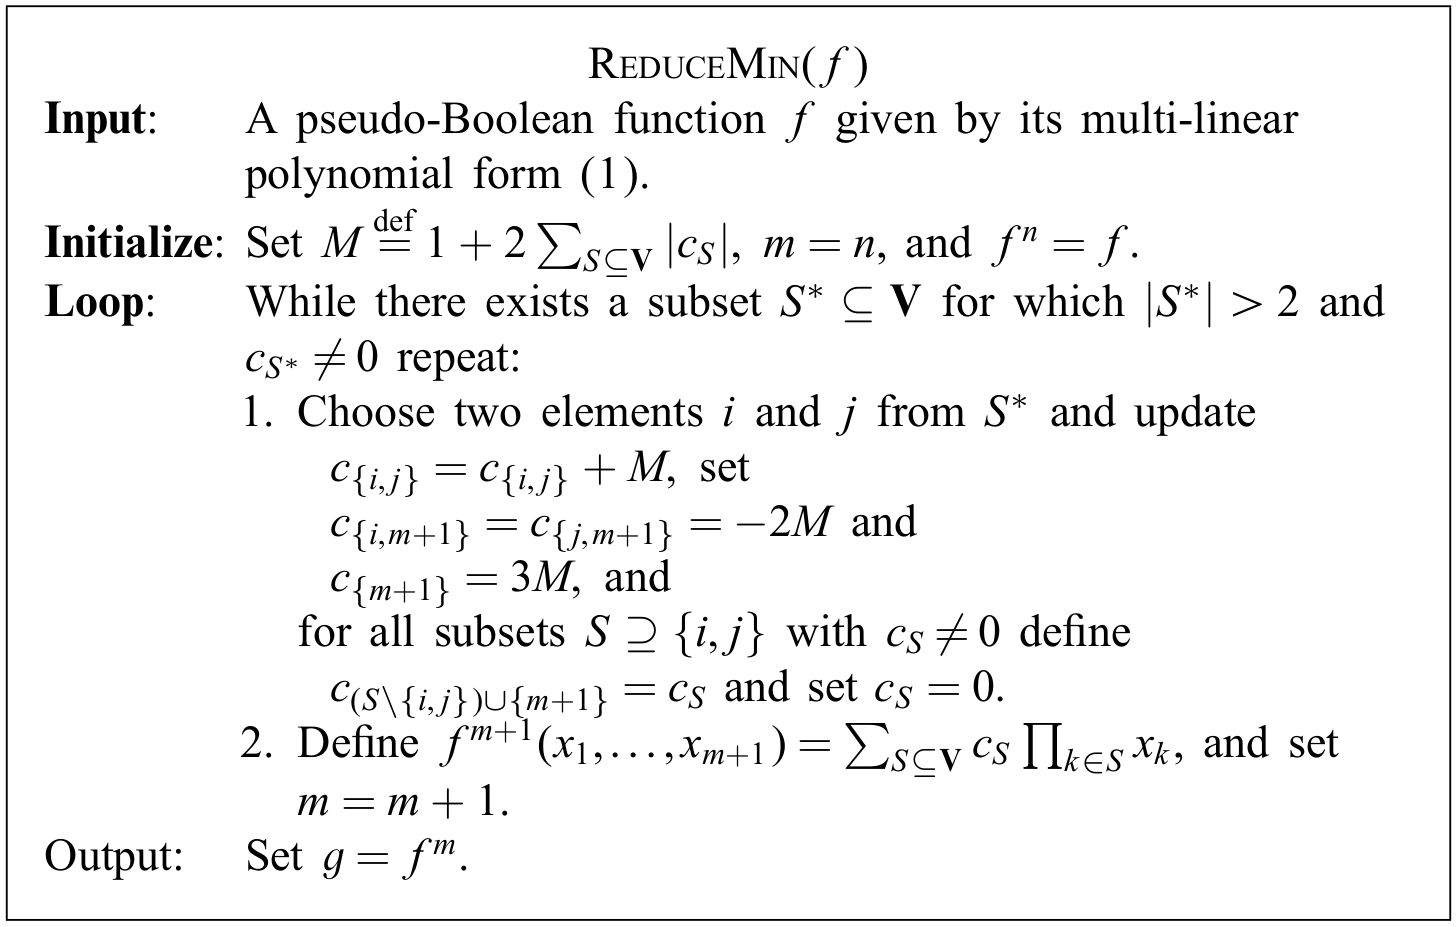
\includegraphics[width=1\textwidth]{images/rosenberg-algo.png}
  \end{center}
\end{frame}
\begin{frame}[t]\frametitle{All circuits solvable with auxiliaries}
  \begin{prop}\label{prop:all-circuits-solvable-with-auxiliaries}
  Let $X \subseteq \bN$ be infinite and $N$, $M$ be finite disjoint subsets. For any choice of $f$, the circuit $(N, M, f)$ is solvable with an Ising system. Since $|X| > |N\cup M|$ in this case, we sometimes say that $X$ is \textbf{solvable with auxiliary spins}.
\end{prop}
Notice that this lemma says nothing about the \textit{number} of auxiliary spins needed to solve a circuit; in general, it can be quite large.
\begin{proof}
  Take the hamming objective function $\text{ham}:\Sigma^{N\cup M} \to \bR$ defined to be the hamming distance from $\sigma$ to the (unique) correct spin state whose $N$ coordinates match those of $\sigma$:
  \begin{align*}
    \text{ham}(\sigma) = d(\sigma_M, f(\sigma_N)).
  \end{align*}
This has minimum value $0$ obtained precisely at spins with correct output coordinates. It is also a pseudo-boolean function and hence can be written uniquely as a multilinear polynomial. Add auxiliary variables until the degree of this polynomial is $2$ using, for instance, Rosenberg reduction. The obtained quadratic will be an Ising Hamiltonian in $|N \cup M \cup A|$ variables where $A$ is the set of auxiliary variables added during the reduction step. 
\end{proof}
\end{frame}
\begin{frame}[t]{References}

\nocite{*}
\printbibliography
\end{frame}

\end{document}
